\chapter{Classificazione}\label{ch:classificazione}

\section{Introduzione}\label{sec:intro-class}
La \textbf{classificazione} suddivide un insieme di dati in \emph{classi} note a priori (etichette),
apprendendo da esempi etichettati come assegnare la classe a nuove tuple. È quindi
\emph{apprendimento supervisionato}. Al contrario, il \emph{clustering} non parte da etichette
(\emph{unsupervised}) e scopre gruppi per similarità.

\paragraph{Predizione (regressione).}
Quando il target è \emph{numerico continuo}, il compito è di \emph{predire} un valore reale
(apprendimento supervisionato \emph{continuo}), cercando una funzione che approssimi
il target, non un confine tra classi.

\subsection{Schema generale di un classificatore}\label{subsec:schema-class}
\begin{enumerate}
  \item \textbf{Costruzione del modello} (training): si apprende da un \emph{training set} etichettato.
  \item \textbf{Validazione/valutazione} (test): si misura la bontà su un \emph{test set} etichettato.
  \item \textbf{Uso} (deploy): si applica il modello a nuove tuple per predirne la classe.
\end{enumerate}

\paragraph{Overfitting.}
L’overfitting si verifica quando un modello “impara a memoria” il training, compreso il rumore: va molto bene sui dati visti ma generalizza male su dati nuovi. In pratica è un segnale che il modello è troppo complesso rispetto alle informazioni disponibili. Per ridurlo, si separano chiaramente i dati per la verifica e si preferiscono soluzioni più semplici quando offrono prestazioni simili.

\begin{figure}[htbp]
  \centering
  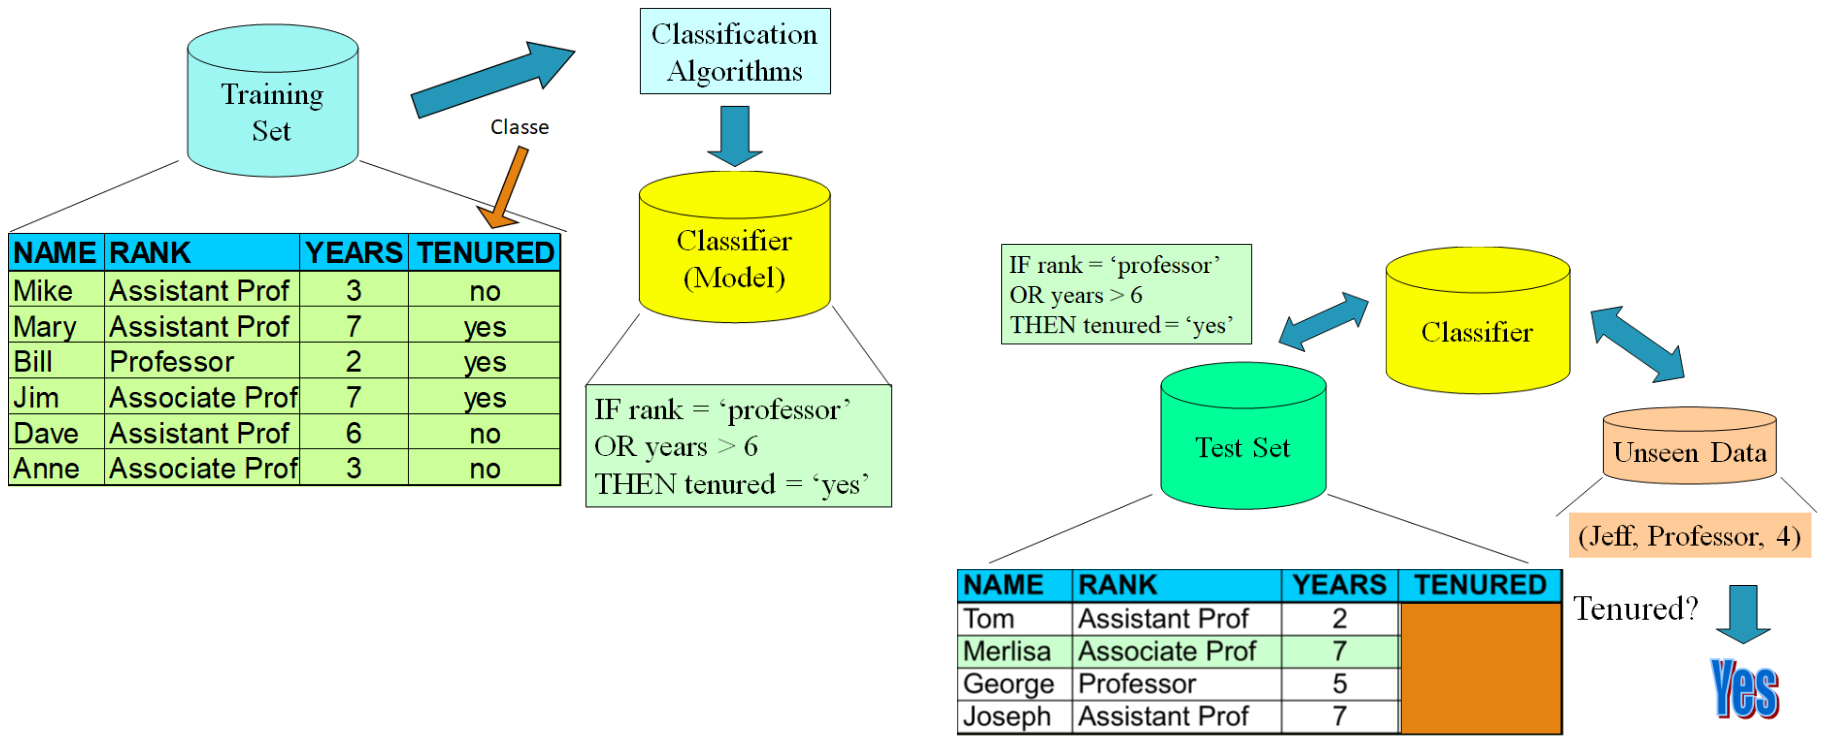
\includegraphics[width=.72\textwidth]{images/schema_classificatore.png}
  \caption{Schema a blocchi di un classificatore: addestramento, validazione e uso.}
  \label{fig:schema-class}
\end{figure}

\subsection{Requisiti desiderabili}\label{subsec:req}
\begin{itemize}
  \item \textbf{Accuratezza}: corretta predizione delle classi (o del valore, per i predittori).
  \item \textbf{Velocità}: tempi di training e di classificazione contenuti.
  \item \textbf{Robustezza}: tolleranza a rumore e dati mancanti.
  \item \textbf{Scalabilità}: efficienza su dataset di grandi dimensioni.
\end{itemize}

% ==========================================================
\section{Alberi decisionali}\label{sec:trees}
Gli \textbf{alberi decisionali} classificano applicando test su attributi lungo i nodi interni;
le \emph{foglie} portano le etichette di classe.

\subsection{Classificazione tramite albero}\label{subsec:tree-class}
La classe di una tupla $q$ si ottiene seguendo il cammino radice$\to$foglia guidato
dai test. Ogni cammino implementa una regola \texttt{IF-THEN} (le condizioni interne sono congiunte in AND). L’insieme di regole è \emph{esaustivo} e \emph{mutuamente esclusivo} (ogni tupla è coperta da una sola regola).

\begin{figure}[htbp]
  \centering
  \begin{minipage}[t]{.50\textwidth}
    \centering
    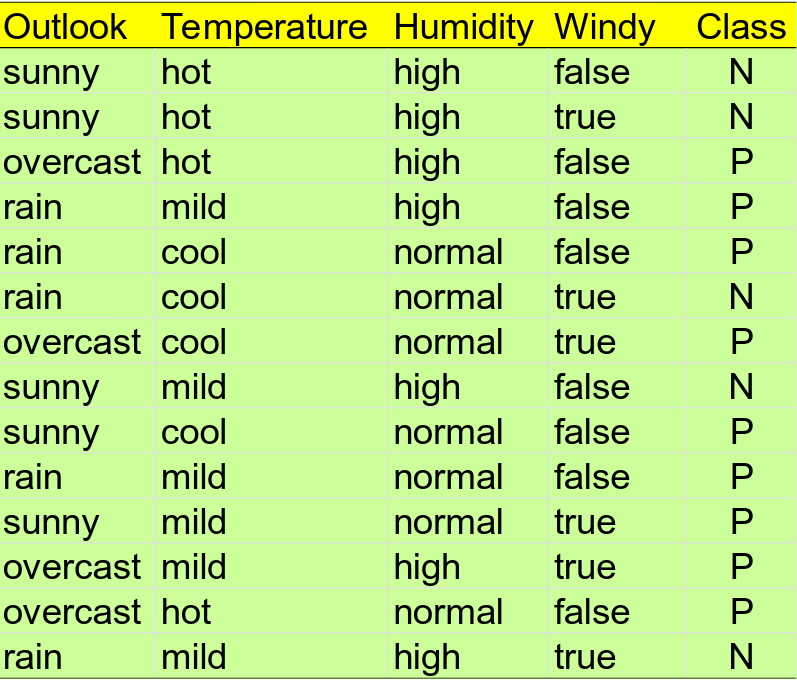
\includegraphics[width=\linewidth]{images/weather_table.png}
  \end{minipage}\hfill
  \begin{minipage}[t]{.48\textwidth}
    \centering
    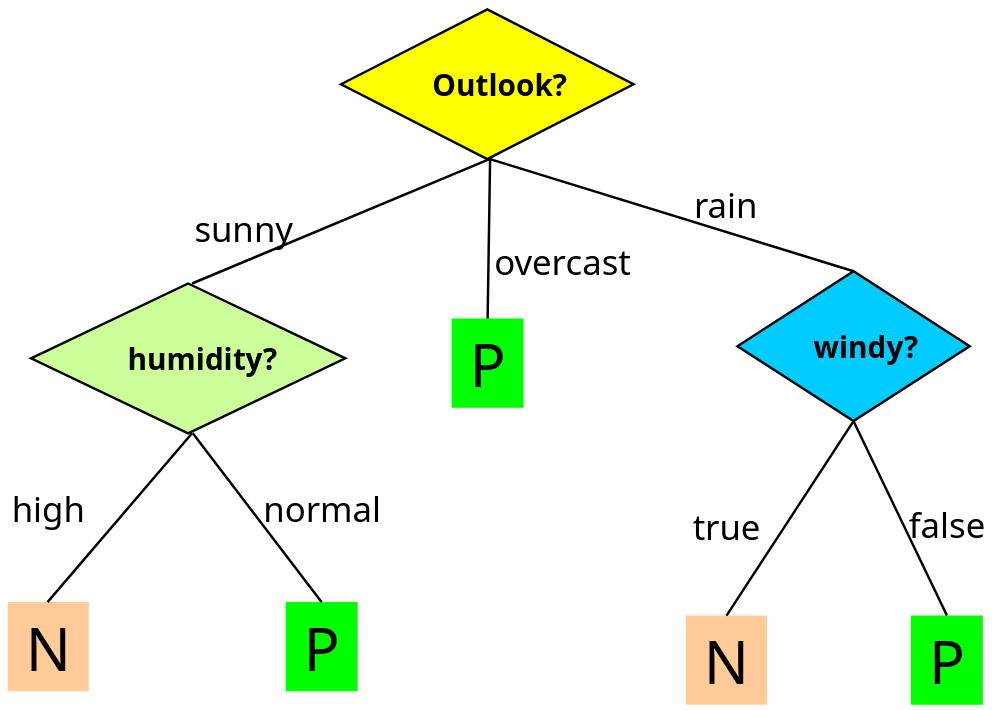
\includegraphics[width=\linewidth]{images/decision_tree_weather.png}
  \end{minipage}
  \caption{Dataset \emph{weather} (a sinistra) e albero decisionale appreso (a destra). 
  La tabella contiene 14 esempi con quattro attributi descrittivi (\texttt{Outlook}, \texttt{Temperature}, 
  \texttt{Humidity}, \texttt{Windy}) e la classe binaria \texttt{P/N}. 
  L’albero (stile ID3/C4.5) sceglie come radice \texttt{Outlook}; il ramo \texttt{overcast} porta 
  direttamente alla classe \texttt{P}, mentre per \texttt{sunny} si testa \texttt{Humidity} e per \texttt{rain} 
  si testa \texttt{Windy}. L’esempio illustra il passaggio da dati tabellari a regole interpretabili.}
  \label{fig:weather-tree}
\end{figure}


\newpage
\subsection{Costruzione top–down}\label{subsec:topdown}
Costruzione ricorsiva dalla radice:
\begin{enumerate}
  \item Se tutte le tuple del nodo $X$ hanno la \emph{stessa} classe $C$, crea una foglia $C$.
  \item Altrimenti scegli un attributo $A$ (non ancora usato) e \emph{ramifica} $X$ (\emph{splitting}) secondo i valori/soglia di $A$; crea i figli.
  \item Per ogni figlio $X_i$: se puro, fermati; se impuro, ripeti ricorsivamente.
\end{enumerate}

\paragraph{Pruning.}
Se le tuple nel nodo sono poche o la profondità è elevata, si può fermare prima e rendere il nodo una foglia (classe di maggioranza, oppure distribuzione di classe).

\subsection{Splitting degli attributi}\label{subsec:splitting}
\begin{itemize}
  \item \textbf{Booleani/numerici}: split \emph{binario} su soglia $t$ (``$\le t$'' a sinistra, ``$>t$'' a destra).
  \item \textbf{Categoriali}: split \emph{binario} definendo un sottoinsieme non vuoto di valori (a sinistra se il valore \emph{non} appartiene al sottoinsieme, a destra altrimenti).
\end{itemize}

\subsection{Scelta dell’attributo e strategia greedy}\label{subsec:greedy}
L’albero minimale è un problema \emph{NP-hard}; si usa una strategia \emph{greedy} che, ad ogni passo, seleziona l’attributo con massima \emph{goodness} (partizioni più pure),
costruendo l’albero “più compatto” possibile.

\subsection{Misure di goodness: Information Gain (ID3)}\label{subsec:ig}
Sia $S_X$ l’insieme di tuple al nodo $X$, con due classi $P$ e $N$; si indichino con $p$
e $n$ le rispettive numerosità. L’\textbf{entropia} di $S_X$ è
\[
H(S_X)\;=\; -\frac{p}{p+n}\log_2\!\frac{p}{p+n}\;-\;\frac{n}{p+n}\log_2\!\frac{n}{p+n}.
\]
Sia $A$ un attributo con $k$ valori distinti, che induce la partizione
$S_X \to S_1,\dots,S_k$. Se $S_i$ contiene $p_i$ e $n_i$ elementi, allora
\[
H(S_i)\;=\; -\frac{p_i}{|S_i|}\log_2\!\frac{p_i}{|S_i|}\;-\;\frac{n_i}{|S_i|}\log_2\!\frac{n_i}{|S_i|},\qquad
\overline{H}_A(S_X)\;=\;\sum_{i=1}^k \frac{|S_i|}{|S_X|}\,H(S_i).
\]
L’\textbf{information gain} dello split su $A$ è
\[
\mathrm{Gain}(S_X,A)\;=\;H(S_X)\;-\;\overline{H}_A(S_X).
\]
Si sceglie l’attributo con gain massimo.

\subsection{Esempio e limitazioni}\label{subsec:ig-example}
Sul dataset “weather” (Fig.~\ref{fig:weather-tree}) si ottengono:
\[
\mathrm{Gain}(\textit{outlook})=0.246,\quad
\mathrm{Gain}(\textit{temperature})=0.029,\quad
\mathrm{Gain}(\textit{humidity})=0.151,\quad
\mathrm{Gain}(\textit{windy})=0.048.
\]
\noindent
\textbf{Limite noto.} L’Information Gain è \emph{sbilanciato} verso attributi con molti valori:
un attributo quasi univoco (es.\ \texttt{ID}) produce molte partizioni piccole (foglie pure),
abbattendo l’entropia media e gonfiando artificialmente il gain, pur senza reale capacità
predittiva.

\begin{figure}[htbp]
  \centering
  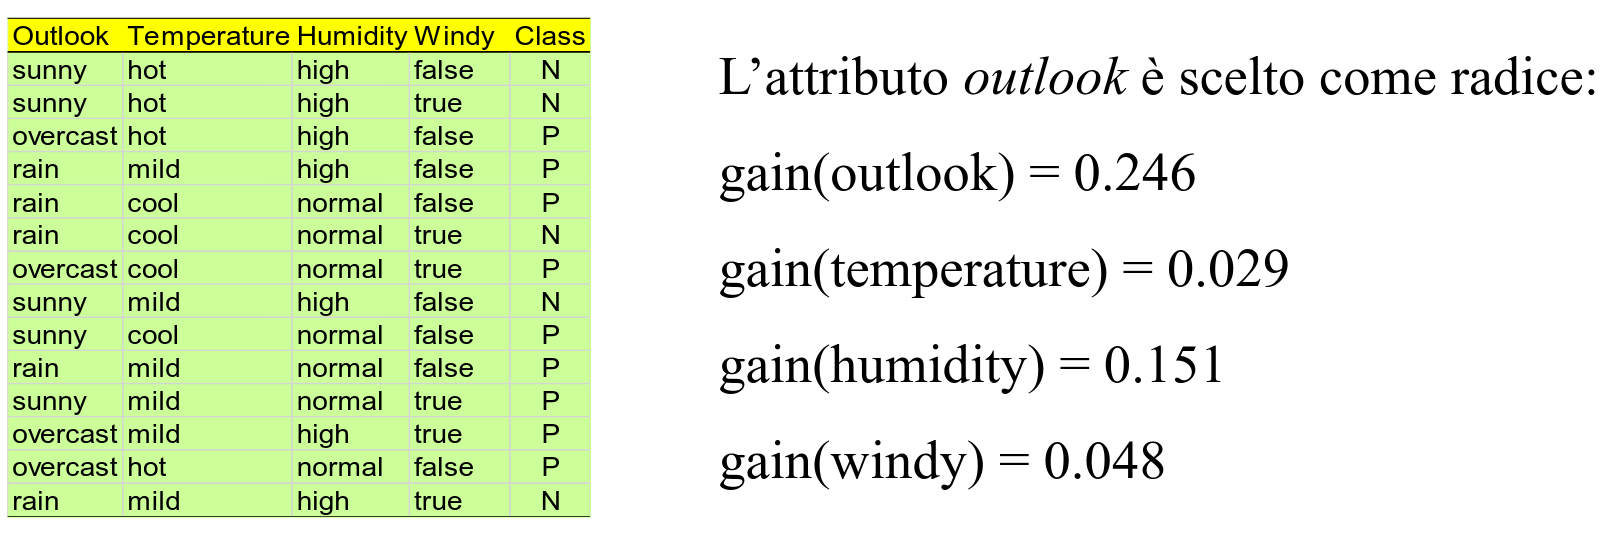
\includegraphics[width=.75\textwidth]{images/ig_outlook_example.png}
  \caption{Esempio di scelta della radice con Information Gain sul dataset “weather”.}
  \label{fig:ig-weather}
\end{figure}
